\section{Evaluation Metrics} \label{eval}

Text-to-SQL tasks can be evaluated by multiple methods: Component Matching, Accurate matching rate and Execution accuracy rate. Predicted SQL statements are compared with standard statements to determine how accurate the match is.
By splitting the predicted SQL statement and definitive statement into multiple clauses according to keywords, we can solve the problem of matching errors caused by the order of the where clause. The matching is successful as long as the elements in both sets are the same.

% pics/acc1.png
\begin{figure}[htb]
    \centering
    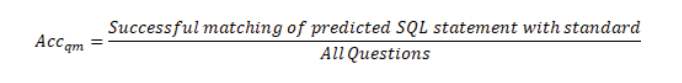
\includegraphics[width=0.6\textwidth]{pics/acc1.png}
    % \caption{Accurate matching rate}
    \label{fig:acc1}
\end{figure}

When using the correct predicted SQL statements, the correct execution rate refers to the proportion of questions that can receive the correct answers from the database.

% pics/acc2.png
\begin{figure}[htb]
    \centering
    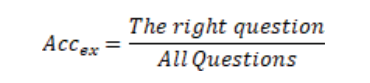
\includegraphics[width=0.4\textwidth]{pics/acc2.png}
    % \caption{Accuracy rate of the predicted SQL statements}
    \label{fig:acc2}
\end{figure}

% By predicting the key F1 values for SQL statements, the model can also be evaluated.

% % pics/f1.png
% \begin{figure}[htb]
%     \centering
%     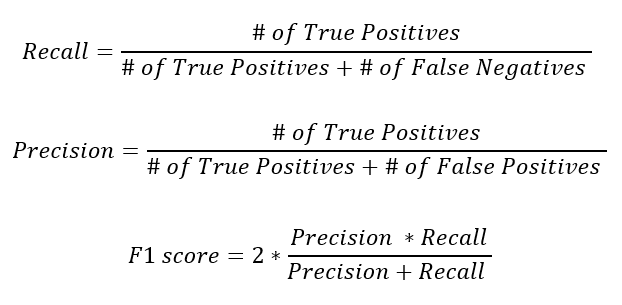
\includegraphics[width=0.6\textwidth]{pics/f1.png}
%     % \caption{F1 score for SQL statements}
%     \label{fig:f1}
% \end{figure}

\subsection{Exact Matching}

Exact Matching\cite{xu_sqlnet_2017}, a popular metric for assessing the effectiveness of Text-to-SQL models, has drawbacks because it can yield erroneous negative results when the semantic parser can produce innovative syntactic structures. The predicted SQL query is compared against the corresponding reference SQL query. The model is considered to have produced the proper SQL query and is given a score of 1.0 if the predicted query is an exact duplicate of the reference query. The model is deemed to have generated an invalid query and obtains a score of 0.0 if the predicted query does not match the reference query. This metric aids in evaluating the overall syntactic and semantic accuracy of the generated query, but it ignores the query's constituent parts. This measure is a reliable evaluation technique because it verifies the entire SQL query. It is, therefore, a more stringent evaluation metric because it only deems a query correct if it exactly matches the reference question, down to the capitalization, spacing, and word order.


\subsection{Exact Set Matching}

Exact Set Matching compares the set of predicted SQL queries with the set of corresponding reference SQL queries, regardless of the elements' order, to assess the performance of a model. If every element from the set of predicted queries is included in the reference query, it returns a score of 1.0; otherwise, it returns a score of 0.0.

Generally, Exact Set Matching is more forgiving than Exact Matching, as the former does not take the order of elements or capitalization into account. On the other hand, Exact Matching is more stringent as it requires a perfect match including the order of words, capitalization and spaces, thus making it a reliable evaluation method.


\subsection{Component Matching}

Component matching\cite{yu_spider_2019} involves comparing the elements of the generated SQL query (e.g., the specified columns and tables) to the elements of the reference SQL query. Evaluation is based on the number of components that match correctly between the produced and reference queries, with a higher amount indicating improved performance. This metric assists in measuring the precision of the model's capability to create the correct SQL query components, but it does not factor in the full syntactic or semantic correctness of the query. Furthermore, it is utilized to assess the performance of various models on the same dataset.

\subsection{Execution Accuracy}

The execution accuracy metric\cite{yu_spider_2019} is a commonly used measure to evaluate the performance of text-to-SQL models. It determines the percentage of correctly generated SQL queries that can be successfully executed on the relevant database. In other words, it evaluates how well a model can convert text written in natural language into a SQL query that can successfully access the desired data from a database.

Execution accuracy is typically reported as a percentage, and higher values denote better performance. It is also important to remember that this metric only considers how correctly the generated SQL queries are syntactically and semantically and ignores how relevant or comprehensive the information is that is returned. Consequently, it is frequently combined with other metrics, such as informativeness, which assesses the accuracy and completeness of the retrieved data.

% \subsection{Distilled Test Suites}

% Distilled Test Suites proposes a method for approximating the semantic accuracy of Text-to-SQL models using test suite accuracy. The method involves creating a small test suite of databases that achieve high code coverage for the gold query from a large number of randomly generated databases. At evaluation time, the denotation accuracy of the predicted queries on the distilled test suite is calculated, providing an efficient upper bound for semantic accuracy. The authors use this method to evaluate 21 models submitted to the Spider leader board and find that it is always correct on 100 examples, while the current Spider metric leads to a 2.5\% false negative rate on average and 8.1\% in the worst case. The authors propose a test suite accuracy that efficiently approximates the semantic accuracy of a Text-to-SQL model by checking the denotations of the predicted queries on a compact test suite of databases with high code coverage. They also contribute a method and software to create compact, high-quality test suites for Text-to-SQL semantic evaluation, test suites to reliably approximate semantic accuracy for eleven popular datasets, and a detailed analysis of why current metrics are poor at approximating semantic accuracy.

% We propose using test suite accuracy to approximate semantic accuracy for Text-to-SQL models. Our method distills a small test suite of databases that achieves high code coverage for the gold query from a large number of randomly generated databases. At evaluation time, it computes the denotation accuracy of the predicted queries on the distilled test suite, thus calculating a tight upper-bound for semantic accuracy efficiently. We use our proposed method to evaluate 21 models submitted to the Spider leader board and manually verify that our method is always correct on 100 examples. In contrast, the current Spider metric leads to a 2.5% false negative rate on average and 8.1% in the worst case, indicating that test suite accuracy is necessary.
% Evaluating the semantic accuracy of a Text-to-SQL model is a long-standing problem: we want to know whether the predicted SQL query has the same denotation as the gold for every possible database. “Single” denotation evaluation executes the predicted SQL query on one database and compares its denotation with that of the gold. It might create false positives, where a semantically different prediction (Figure 1 prediction 1) happens to have the same denotation as the gold, on a particular database. In contrast, exact string match might produce false negatives: Figure 1 prediction 2 is semantically equivalent to the gold but differs in logical form.
% However, these representations cannot express sort operations and float comparisons, and hence do not support the full range of operations that Text-to-SQL models can use. We ideally need a method to approximate semantic accuracy reliably without operation constraints.
% If the computational resources were unlimited, we could compare the denotations of the predicted query with those of the gold standard on a large number of random databases (Section 4.1), and obtain a tighter upper bound for semantic accuracy than single denotation evaluation. The software testing literature calls this idea fuzzing (Padhye et al., 2019; AFL; Lemieux et al., 2018; Qui, December 1, 2019).
% We propose a test suite accuracy (Section 2) to efficiently approximate the semantic accuracy of a Text-to-SQL model, by checking the denotations of the predicted queries on a compact test suite of databases with high code coverage. We introduce how to construct and search for such a test suite without prior information about model-predicted queries.
% Our search objective is formally defined through neighbor queries (Section 3.1), which are generated by modifying one aspect of the gold query. For example, prediction 1 in Figure 1 is a neighbor query of the gold, since they differ only by a “WHERE” clause. These neighbor queries are usually semantically different from the gold, and if a test suite can distinguish them from the gold, it is likely to distinguish other wrong queries as well. The latter holds because distinguishing all neighbors from the gold requires executions on these databases to exercise every modified part of the gold query, hence reflecting comprehensive code coverage and high test quality (Miller and Maloney, 1963; Ammann and Offutt). Hence, we formalize our objective as finding a small test suite that can distinguish all the neighbors (Section 3.2).
% We search under this objective by generating a large number of random databases (Section 4.1) and keeping a small fraction of them that can distinguish the neighbors from the gold (Section 4.2). We call this set of databases a distilled test suite.
% While evaluating model-predicted queries, we only check their denotations on the distilled test suite to approximate semantic accuracy efficiently
% We distilled a test suite for the Spider dataset (Yu et al., 2018) (Section 5) from 1000 random databases, which can distinguish more than 99% of the neighbor queries. We used the test suite to evaluate 21 Spider leader board submissions, randomly sampled 100 model-predicted queries where our method disagreed with exact set match (ESM, the current Spider official metric), and manually verified that our method was correct in all these cases.
% To summarize, we contribute:
% - A method and software to create compact, high-quality test suites for Text-to-SQL semantic evaluation.
% - Test suites to reliably approximate semantic accuracy for eleven popular datasets.
% - A detailed analysis of why current metrics are poor at approximating semantic accuracy.
% Computational Efficiency. We minimize the size of S g to speed up test suite evaluations.
% Code Coverage. The test suite needs to cover every branch and clause of the gold query such that it can test the use of every crucial clause, variable, and constant.
% We measure the code coverage of a test suite by its ability to distinguish the gold query from its neighbor queries: a set of SQL queries that are close to the gold in surface forms but likely to be semantically different. To generate them, we modify one of the following aspects of the gold query (Figure 2): (1) replace an integer (float) constant with either a random integer (float) or its value ± 1 (0.001); (2) replace a string with a random string, its sub-string or a concatenation of it with another random string; (3) replace a comparison operator/column name with another; (4) drop a query span unless the span does not change the semantics of the query. For example, the “ASC” keyword does not change the semantics because it is the default sort order. We then remove modified queries that cannot execute without any errors.
% We optimize the above objective through fuzzing: a software testing technique that generates a large number of random inputs to test whether a program satisfies the target property (e.g., SQL equivalence). We describe a procedure to sample a large number of random databases and keep a small fraction of them to distill a test suite S g.
% A database w needs to satisfy the input type constraints of the gold program g, which include using specific table/column names, foreign key reference structure, and column data types. We describe how to generate a random database under these constraints and illustrate it with Figure 3. If a column c1 refers to another column c2 as its foreign key, all elements in c1 must be in c2 and we have to generate c2 first. We define a partial order among the tables: table A < table B if B has a foreign key referring to any column in table A. We then generate the content for each table in ascending order found by topological sort. For example, in Figure 3, we generate the “State” table before the “People” table because the latter refers to the former. We now sample elements for each column such that they satisfy the type and foreign key constraints. If a column c1 is referring to another column c2, each element in c1 is uniformly sampled from c2. Otherwise, if the column is a numerical(string) type, each element is sampled uniformly from [−263, 263] (a random string distribution). We also randomly add in constant values used in g (e.g., 34 and “Alice”) and their close variants (e.g., 35 and “aAlicegg”) to potentially increase code coverage. We denote the database distribution generated by this procedure as Ig.
% We use samples from Ig to construct a small test suite S g such that it can distinguish as many neighbor queries (Section 3.1) in Ng as possible. We initialize S g to be empty and proceed greedily. A database w is sampled from the distribution Ig; if w can distinguish a neighbor query that cannot be distinguished by any databases in S g, we add w to S g. Appendix A.1 gives a more rigorous description. In the actual implementation, we also save the disk space by sharing the same random database wt across all gold SQL queries that are associated with the same schema. Though this algorithm is far from finding the optimal solution to Objective 4, in practice, we find a test suite that is small enough to distinguish most neighbor queries.
% We generate test suites S g for the development set of Spider (Yu et al., 2018), which contains 1034 English utterances and their corresponding SQL queries, spanning across 20 different database schemata. It stratifies data into four categories (easy, medium, hard, and extra-hard) according to difficulty level measured by gold SQL complexity.
% The Spider official evaluation metric is exact set match (abbreviated as ESM) (Zhong et al., 2017; Yu et al., 2018). It parses the gold and model predicted queries into sub-clauses and determines accuracy by checking whether they have the same set of clauses. It improves over exact string matching by preventing false negatives due to semantically equivalent clause reordering. However, it is still considered a strict metric and creates false negatives. 
% To further reduce false negatives, the actual implementation of the official Spider metric is looser. We list all of its major differences from the standard ESM below; accordingly, we either adapt our test suite evaluation or fix the Spider implementation to make a fair comparison. 
% (1) The Spider metric does not check constant prediction correctness. Therefore, our adapted test suite evaluation enumerates all possible ways to replace the constants in a model-predicted query with the gold constants and consider a model-predicted query to be correct if one of the replacements passes the test suite. (2) The Spider metric does not check column order, so our adapted evaluation considers two denotations equivalent if they only differ by column order. (3) The Spider evaluation script accidentally ignores any join predicate. We fix this bug. (4) The Spider metric does not check table variable names. Yu et al. (2018) implemented this because different intermediate tables can contain the same column, hence selecting any of them is equivalent. We keep this feature since it effectively rules out many false negatives. However, it also introduces new false positives (e.g., Figure 8 row 1). Unless we explicitly specify, in the rest of our paper, “ESM” and “test suite accuracy” refer to these adapted metrics rather than the original ones.
% Given that test suite evaluation empirically provides an improved approximation of semantic equivalence, we use test suite accuracy as ground truth and retrospectively examine how well ESM approximates semantic accuracy. We calculate the false positive/false negative rate for each difficulty split and report the mean, standard deviation, and max for all 21 submissions.
% We plot ESM against test suite accuracy for all 21 dev set submissions in Figure 6. On a macro level, ESM correlates well with test suite accuracy with a Kendall τ correlation of 91.4% in aggregate; however, the correlation decreases to 74.1% on the hard fraction. Additionally, ESM and test suite accuracy start to diverge as model performance increases. These two facts jointly imply that, as models become better at harder queries, ESM is no longer sufficient to approximate semantic accuracy. On a micro level, when two models have close performances, improvements in semantic accuracy might not be reflected by increases in ESM.
% Although test suite evaluation consumes more space and computational resources than single denotation evaluation, it is parallelizable and affordable by most researchers. We may speed up the evaluation by checking denotation only on a single database sampled from the distribution Ig. While this sped-up version sacrifices precision for speed, retrospectively, it produces the exact same outcomes as running the full test suite on the 21 submissions. Therefore, the sped-up version might be useful when occasional errors are tolerable (e.g. denotation based training). However, we still recommend using the full test suite for reliable evaluation, since a single sample from Ig cannot distinguish all neighbors, and checking denotations on multiple databases with comprehensive code coverage is always more reliable, especially when we have no prior information about the model-predicted queries.
% **False Positives** Although standard ESM is strict, the adapted ESM (Section 5.3) can introduce false positives because it ignores table variable names. See Figure 8 row 1 for an example.
% **False Negatives** Row 2-4 shows that slightly complicated queries usually have semantically equivalent variants, and it is nontrivial to tell whether they are semantically equivalent unless we execute them on a test suite or manually verify.
% Nevertheless, even though test suite accuracy reliably approximates semantic accuracy according to our observation, researchers might also care about other aspects of a model-predicted query. Semantic accuracy is only concerned with what are the denotations of a query, but not how it calculates them. For example, Figure 8 row 5 represents one of the most common types of false negatives, where the model-predicted query chooses to join other tables even though it is unnecessary. While semantically correct, the model-predicted query increases running time. Figure 8 row 7 exhibits a similar but more complicated and rarer example. Inserting gold values into model-predicted queries as described in Section 5 might also unexpectedly loosen the semantic accuracy metric. For example, in Figure 8 row 6, the model-predicted query uses the “LIKE” keyword rather than the “=” operator. By SQL style conventions, “LIKE” usually precedes a value of the form “%[name]%” and corresponds to natural language query “contains [name]” rather than “matches [name]”; it seems plausible that the model does not understand the natural language query. However, if we replace the wrong value “%[name]%” with the gold value “[name]” after the “LIKE” operator, the predicate becomes semantically equivalent to “= [value]” and hence makes the query semantically correct. Value prediction is a crucial part of evaluating Text-to-SQL models.
% We propose test suite accuracy to approximate the semantic accuracy of a Text-to-SQL model, by automatically distilling a small test suite with comprehensive code coverage from a large number of random inputs. We assure test suite quality by requiring it to distinguish neighbor queries and manually examining its judgments on model-predicted queries. Our test suites will be released for eleven datasets so that future works can conveniently evaluate test suite accuracy. This metric better reflects semantic accuracy, and we hope that it can inspire novel model designs and training objectives.
% We do not attempt to solve SQL equivalence testing in general. While our test suite achieves comprehensive code coverage of the gold query, it might not cover all the branches of model-predicted queries. Adversarially, we can always construct a query that differs from the gold only under extreme cases and fools our metric. Fortunately, we never observe models making such pathological mistakes. However, it is necessary to revisit and verify this hypothesis at some point in the future due to Goodhardt's Law, since researchers will optimize over our metric.
% Although test suite evaluation can never create false negatives in a strict programming language sense, it might still consider "acceptable answers" to be wrong and result in false negatives in a broader sense. For example, in a database of basketball game results, the predicate "A wins" is equivalent to "scoreA > scoreB" according to common sense. However, such a relation is not explicitly reflected in the database schema, and our procedure might generate an "unnatural" database where "scoreA > scoreB" but not "A wins", hence distinguishing the model-predicted query from the gold. Fortunately, this issue is mitigated by current models. If "A wins" is mentioned in the text, the model would prefer predicting "A wins" rather than "scoreA > scoreB". Nevertheless, to completely solve this issue, we recommend that future dataset builders explicitly define the database generation procedure. Automatic constraint induction from database content and schema descriptions might also be possible, which is an open research problem in its own right.
